% !TeX root = ../libro.tex
% !TeX encoding = utf8

\setchapterpreamble[c][0.75\linewidth]{%
	\sffamily
  Definiremos los modelos utilizados en el trabajo. 
	\par\bigskip
}
\chapter{Aprendizaje automático}\label{ch:machine-learning}
El aprendizaje automático es una aplicación de la inteligencia artificial que provee al sistema de la habilidad para aprender automáticamente y mejorar con la experiencia sin ser explícitamente programado para ello (Arthur Samuel, 1959). Hace uso de los algoritmos de aprendizaje que son algoritmos que estiman una dependencia desconocida entre los datos de entrada y de salida de un sistema desde unas muestras conocidas. Una vez esta dependencia ha sido estimada, se puede usar para predecir las futuras salidas del sistema a partir de los valores de entrada conocidos.\\
Hay tres tipos de aprendizajes:
\begin{itemize}
  \item Aprendizaje \textbf{supervisado}: Es el tipo de aprendizaje más utilizado. Se aplica a datos \textbf{etiquetados}. Tiene como objetivo aprender la función desconocida que asigna los datos con las etiquetas minimizando una función de error. lo usaremos para nuestro conjunto de datos, pues es etiquetado.
  \item Aprendizaje \textbf{no supervisado}: Se usa para los datos no etiquetados y se pretende buscar patrones o relaciones entre los datos. Un ejemplo típico de este tipo de aprendizaje es el de \textbf{agrupamiento} o \textit{clustering} que busca agrupar los datos según algún patrón o relación.
  \item Aprendizaje \textbf{por refuerzo}: En vez de ser etiquetado, da solo una indicación de si la predicción es correcta o no mediante alguna recompensa o penalización en función de las acciones que haga.
\end{itemize}
\cite{jordan2015machine}\\
\section{Esquema básico de aprendizaje}
Un primer ejemplo y esquema de aprendizaje automático sería el siguiente, supongamos que hay un banco que recive miles de solicitudes para una tarjeta de crédito y quiere automatizar el proceso. No se conoce ninguna fórmula para aceptar o denegar una tarjeta pero se dispone de gran cantidad de datos de los aplicantes: información personal, sueldo, prestamos pendientes y más información relacionada al crédito, así que se usan estos datos para encontrar una fórmula adecuada.\\
Así, se tiene la entrada \textbf{x} (información del cliente), la función desconocida ideal para llevar a cabo la decisión $f:X \rightarrow Y$, donde $X$ es el espacio de la entrada (conjunto de las posibles entradas de \textbf{x}), e $Y$ es el espacio de la salida (conjunto de todas las posibles salidas, en este caso una decisión de sí o no). Se denotará al set de datos por $D$, con ejemplos de entrada-salida $(x_{1},y_{1}),...,(x_{N},y_{N})$ donde $y_{n}=f(x_{n})$ para $n=1,...,N$. Los ejemplos se suelen llamar observaciones. Por último, hay un algoritmo de aprendizaje que aproxima $h:X \rightarrow Y$ a $f$.  El algoritmo elige $h$ de entre un conjunto de funciones candidatas o hipótesis, $H$, como por ejemplo el conjunto de todas las funciones lineales.\\
El banco usará la función $h$ para hacer la decisión puesto que la $f$ ideal no la tiene así que el algoritmo elige la $h$ que mejor aproxima $f$ en un conjunto de \textit{entrenamiento} o \textit{training} de anteriores clientes. \cite{abu2012learning}\\
La siguiente figura ilusta esquemáticamente el problema de aprendizaje:
\begin{figure}[H]
  \centering
  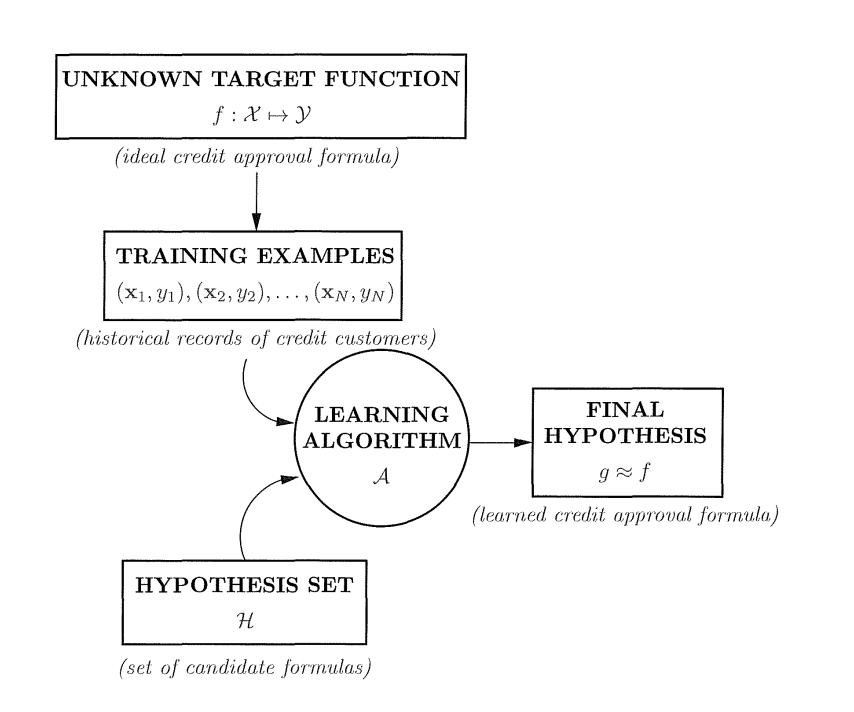
\includegraphics[width=0.65\textwidth]{Problema_aprendizaje_basico}
  \caption{Esquema básico de aprendizaje.}
  \label{fig:k-nn-example}
\end{figure}

Para este trabajo, $X=\mathbb{R}^{d}$, siendo $\mathbb{R}^{d}$ un espacio euclídeo d-dimensional, con las coordenadas descritas en el \autoref{ch:base-datos} siendo cada columna una coordenada, $Y=\lbrace 0,2 \rbrace$ una decisión binaria de si el individuo es sano o afectado (o padre de afectado para el estudio con controles).\\
\section{Errores}
También hay que tener en cuenta dos conceptos importantes: los errores. Hay de dos tipos, el primero es el error dentro de la muestra definido como la fracción de $D$ donde $f$ y $h$ no concuerdan:
\[E_{in}(h) = \frac{1}{N}\sum_{n=1}^{N}[[h(x_{n}) \neq f(x_{n})]]\]
donde el operador [[$\cdot$]]=1 si lo de dentro se cumple y 0 en caso contrario. Análogamente también está el error fuera de la muestra:
\[ E_{out}(h)=\mathbb{P}[h(x) \neq f(x)] \]
la probabilidad está basada en la distribución de $X$ que se susa para muestrear.\\
Para cuantificar la relación que existe entre estos dos errores, se usa la \textit{desigualdad de Hoeffding} que provee de una cota superior de la probabilidad de que la suma de variables aleatorias independientes y acotadas se desvíe de su valor esperado más de una cierta cantidad. Esta desigualdad indica que para cualquier tamaño de muestra N,
\[ \mathbb{P}[\vert E_{in}(h)-E_{out}(h) > \epsilon] \leq  2e^{-2\epsilon^{2}N} \quad \forall \epsilon > 0 \]
El error dentro de la muestra $E_{in}$ es una variable aleatoria que depende de la muestra y el error fuera de la muestra $E_{out}$ es desconocido pero no aleatorio. Ahora bien, esto ocurre bajo el supuesto de que $h$ está fija y es una en particular antes de generar el conjunto de datos. \cite{abu2012learning}
\subsection{Generalización de errores I}
Para solucionar que $h$ tenga que estar \textbf{fija}, consideramos un conjunto de hipótesis $H$ y asumimos primero que tien un número finito de hipótesis $H=\lbrace h_{1},...,h_{M}$. El objetivo es poder poner el límite a una hipótesis $g$ de $H$ que no esté fija antes de generar los datos, porque la hipótesis seleccionada $g$ depende de los datos. Así que vamos a intentar limitar $\mathbb{P}[\vert E_{in}(g)-E_{out}(g) \vert > \epsilon]$ de forma que no dependa de la $g$ que el algoritmo de aprendizaje elija. Como $g$ es una de las hipótesis independientemente del algoritmo y de la muestra, siempre es verdad que:
"$\vert E_{in}(g)-E_{out}(g) \vert > \epsilon$" $\Longrightarrow$ "$\vert E_{in}(h_{1})-E_{out}(h_{1}) \vert > \epsilon$ \textbf{or} $\vert E_{in}(h_{2})-E_{out}(h_{2}) \vert > \epsilon$ \textbf{or} ... \textbf{or} $\vert E_{in}(h_{M})-E_{out}(h_{M}) \vert > \epsilon$".\\
Llamemos $\mathcal{B}_{1}$ a la parte izquierda de la implicación anterior y $\mathcal{B}_{2}$ a la parte derecha.$\mathcal{B}_{2}$ tiene la propiedad deseada: las hipótesis $h_{m}$ están fijas, y aplicamos dos reglas básicas de probabilidad:
\[ \textnormal{si } \mathcal{B}_{1} \Longrightarrow \mathcal{B}_{2} \textnormal{ entonces } \mathbb{P}[\mathcal{B}_{1}] \leq \mathbb{P}[\mathcal{B}_{2}]\]
y que si $\mathcal{B}_{1},\mathcal{B}_{2},...,\mathcal{B}_{M}$ son cualesquiera eventos, entonces:
\[ \mathbb{P}[\mathcal{B}_{1} \textnormal{ or } ... \textnormal{ or } \mathcal{B}_{M}] \leq \mathbb{P}[\mathcal{B}_{1}]+...+\mathbb{P}[\mathcal{B}_{M}] \]
Tenemos con estas dos propiedades que:
\[ \mathbb{P}[\vert E_{in}(g)-E_{out}(g) \vert > \epsilon] \leq \mathbb{P}[\vert E_{in}(h_{1})-E_{out}(h_{1}) \vert > \epsilon \textnormal{\textbf{ or }} \vert E_{in}(h_{2})-E_{out}(h_{2}) \vert > \epsilon \textnormal{\textbf{ or }} ...\]
\[\textnormal{\textbf{ or }} \vert E_{in}(h_{M})-E_{out}(h_{M}) \vert > \epsilon] \leq \sum_{m=1}^{M}\mathbb{P}[\vert E_{in}(h_{m})-E_{out}(h_{m}) \vert > \epsilon] \]
Aplicando la desigualdad de Hoeffding a los M términos de la sumatoria obtenemos el resultado deseado:
\[ \mathbb{P}[\vert E_{in}(g)-E_{out}(g) \vert > \epsilon] \leq 2Me^{-2\epsilon^{2}N} \]
Como se puede ver, esto funciona cuando M es finita. \cite{abu2012learning}
\subsection{Generalización de errores II}
Para terminar esta sección se va a definir la \textit{función de crecimiento} o, más conocida en inglés, \textbf{\textit{growth function}} que formaliza el número efectivo de hipótesis.\\
Antes vamos a convertir la formula $\mathbb{P}[\vert E_{in}(g)-E_{out}(g) \vert > \epsilon] \leq 2Me^{-2\epsilon^{2}N}$ en algo más conveniente. Tomamos un \textit{nivel de tolerancia} $\delta$ y afirmamos con una probabilidad de al menos $1 - \delta$ que:
\[ E_{out} \leq E_{in}(g) + \sqrt{\frac{1}{2N} ln \frac{2M}{\delta}} \] 
A esta cota se la llama \textit{cota de generalización} pues acota $E_{out}$ en términos de $E_{in}$. Se ha conseguido la expresión de la siguiente forma: con al menos una probabilidad de $1 - 2Me^{-2N \epsilon^{2}}$, $\vert E_{out} - E_{in} \vert \leq \epsilon $ lo que implica que $E_{out} \leq E_{in} + \epsilon$. Escribimos $\delta = 2Me^{-2N\epsilon^{2}}$, de donde $\epsilon=\sqrt{\frac{1}{2N}ln\frac{2M}{\delta}}$ y se deduce la cota de generalización.
\begin{definicion}
Sean $x_{1},...,x_{N} \in X$. La dicotomía generada por H en estos puntos está definida por  \[ H(x_{1},...,x_{N})= \lbrace (h(x_{1}),...,h(x_{n})) \vert h \in H \rbrace \]
\end{definicion}
Es una dicotomía pues separa $x_{1},...,x_{n}$ en dos grupos: los que su $h$ vale 1 y los que vale -1, así, cuanto mayor es la dicotomía, más 'diversa' es $H$.
\begin{definicion}
La \textbf{función de crecimiento} está definida por un conjunto de hipótesis $H$ por \[ m_{H}(N)=\max_{x_{1},...,x_{N} \in X} \vert H(x_{1},...,x_{N}) \vert \]
donde $\vert \cdot \vert$ indica la cardinalidad del conjunto.
\end{definicion}
En otras palabras, $m_{H}(N)$ es el máximo número de dicotomías que pueden ser generadas por $H$ en cualquiera $N$ puntos.\\
Para cualquier $H$, como $H(x_{1},...,x_{N}) \subseteq \lbrace -1,+1 \rbrace$, el valor de $m_{H}(N)$ es como mucho $\vert \lbrace -1,+1 \rbrace \vert$, así que $m_{H}(N) \leq 2^{N}$. Por intuición se puede afirmar que $m_{H}(N)$ crece más rápido cuanto más compleja se vuelve $H$, que es lo que se espera ya que es lo que va a reemplazar a M en la cota de generalización. Si $H$ es capaz de generar todas las posibles dicotomías en la muestra, se dice que \textit{separa}, o en inglés \textbf{\textit{shatter}}, $x_{1},...,x_{N}$\\
Sin embargo, no es práctico computar $m_{H}$ para cada conjunto de hipótesis que se use, pero esto no es necesario pues basta con usar una cota superior y la cota de generalización aún se sostendrá y así se hará más facil computar $m_{H}$.
\begin{definicion}
Si el conjunto nungún conjunto de datos de tamaño k puede ser \textit{separado} por $H$, entonces k se dice que es un \textbf{punto de ruptura} para $H$.
\end{definicion}
\cite{abu2012learning}\\
Así, $m_{H} < 2^{k}$ y en general es más fácil de encontrar este punto que de computar la función de crecimiento completa para esa $H$. Lo más importante de este concepto es que si $m_{H}(N)=2^{N}$ rompe en cualquier punto, podemos acotar $m_{H}$ por un polinomio de forma que si se sustituye por $M$ en el \textit{error de generalización} $\sqrt{\frac{1}{2N}ln\frac{2M}{\delta}}$ cuando $N \longrightarrow \infty$ irá a cero, cosa que no pasa sin esa cota polinómica.\\
Ahora se va a probar esa cota polinómica. Introducimos antes un concepto. No depende de $H$ así que la cota será aplicada a cluaquier $H$.
\begin{definicion}
Se denota $B(N,k)$ al número máximo de dicotomías en $N$ puntos tales que ningún subconjunto de tamaño $k$ del de $N$ puntos puede ser \textit{separado} por estas dicotomías.
\end{definicion}
Esta definición asume un punto de ruptura $k$ y está definido como un máximo así que sirve como cota superior para cualquier $m_{H}(N)$ que tenga un punto de ruptura $k$:
\[ m_{H}(N) \leq B(N,k) \textnormal{ si } k \textnormal{ es un punto de ruptura para } H\]
\begin{lema}
(Lema de Sauer) \[ B(N,k) \leq \sum_{i=0}^{k-1} \binom{N}{i} \]
\end{lema}
\begin{proof}
Cuando $k=1$, $B(N,1)=1$ para todo $N$ pues ningún subconjunto de tamaño 1 puede ser separado así que sólo admite una dicotomía así que el lema se cumple. Cuando $N=1$, $B(1,k)=2$ para $k>1$ puesto que no existen subconjuntos de tamaño $k$ así que las dos únicas posibilidades son 1 y -1, con lo que el lema se cumple. Ahora se va a realizar la prueba por inducción, asumimos que es cierto para todo $N \leq N_{0}$ y todo $k$. Necesitamos probar que es verdad para $N=N_{0}+1$ y todo $k$. Como la desigualdad ya es cierta cuando $k=1$ solo hace flata preocuparse por $k \geq 2$. Por definición de B, ocurre que
\[ B(N_{0}+1,k) \leq B(N_{0},k)+B(N_{0},k-1) \]
Aplicando la hipótesis de inducción a cada término de la derecha de la desigualdad se tiene que:
\[ B(N_{0}+1,k) \leq \sum_{i=0}^{k-1} \binom{N_{0}}{i} + \sum_{i=0}^{k-2} \binom{N_{0}}{i} =\] \[ = 1 + \sum_{i=0}^{k-1} \binom{N_{0}}{i} + \sum_{i=0}^{k-1} \binom{N_{0}}{i-1} = 1+ \sum_{i=0}^{k-1} \left[ \binom{N_{0}}{i} + \binom{N_{0}}{i-1} \right] = \] \[ = 1 + \sum_{i=0}^{k-1} \binom{N_{0} + 1}{i} = \sum_{i=0}^{k-1} \binom{N_{0}+1}{i}\]
donde se ha usado la identidad de combinatoria $\binom{N_{0}+1}{i} = \binom{N_{0}}{i}+\binom{N_{0}}{i-1}$. Probado esto, la inducción concluye y el lema es cierto para todo $N$ y $k$.
\end{proof}
\section{Descripción de los modelos utilizados}\label{st:modelos-utilizados}
El problema que se pretende resolver en este trabajo consiste en una predicción de etiquetas, es decir, al uso del aprendizaje supervisado para resolverlo. Dentro del aprendizaje supervisado encontramos varios modelos de gran potencia predictiva como los que describiremos en esta sección.
\subsection{k-Nearest Neighbors}\label{sst:k-nn}
El modelo k-Nearest Neighbours (k-NN) es uno de los modelos más intuitivos y transparentes y se aleja un poco de la idea de aproximar una función ideal para tomar la decisión de clasificación. La idea básica se muestra en la \autoref{fig:k-nn-example}. Se clasificará el vecino desconocido con la clase de los vecinos más cercanos a él, y si hay de varios tipos como en la figura, se puede resolver por simple mayoría o por votación ponderada por distancia, que veremos más adelante. Así que en k-NN se pueden diferenciar dos etapas: primero determinar los vecinos más cercanos y segundo, determinar la clase usando esos vecinos. \cite{padraiddelany2007k}

\begin{figure}[H]
  \centering
  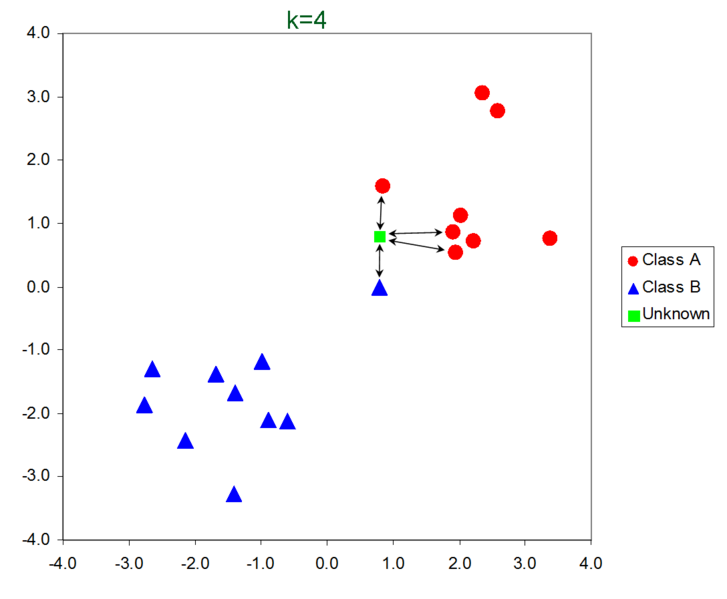
\includegraphics[width=0.4\textwidth]{k-nn-example}
  \caption{Ejemplo de 4-NN.}
  \label{fig:k-nn-example}
\end{figure}
\begin{center}
\cite{peterson2009k}
\end{center}

\subsubsection{Métrica}
Sea $X$=$\lbrace x_{1},...,x_{n} \rbrace$ donde $n=\mid X \mid$ un conjunto de entrenamiento, con x representando las instancias. Las instancias están descritas por un conjunto de variables $F$. Cada instancia de entrenamiento está etiquetada con una etiqueta de clase $y_{i} \in Y$, es decir, la función de etiquetado establece una aplicación biyectiva entre $X$ e $Y$. El objetivo es clasificar un ejemplo desconocido \textbf{$q$}.\cite{padraiddelany2007k}\\
Para cada $x_{i} \in X$ calculamos la distancia como la distancia de :
\[ MD_{p}(\textbf{q},x_{i})= (\sum_{f \in F}  \vert q_{f} - x_{if} \vert ^{p})^{1/p} \quad \cite{inproceedings} \] 
Para p=1 la distancia de Minkowski es la llamada distancia Manhattan, para p=2, la Euclídea y para p=$\infty$ la de Chebychev. Sus expresiones son las que siguen \cite{inproceedings}:
\[ d^{2}(q,x_{i})= (q-x_{i})(q-x_{i})' \quad Euclídea \]
\[ d(q,x_{i})=\sum_{f \in F}  \vert q_{f} - x_{if} \vert \quad  Manhattan \]
\[ d(q,x_{i})=max_{f \in F} \lbrace \vert q_{f} - x_{if} \vert \rbrace \quad Chebychev \]

\subsubsection{Votación}
La votación consiste en establecer un criterio para asignar a $q$ una de las etiquetas de $Y$. Esto puede hacerse asignando la etiqueta que tengan la mayoría de vecinos más cercanos a $q$ o también puede establecerse una función de votación. La más usual es establecer la votación en función de la inversa de la distancia entre $q$ y sus vecinos. 
\[ Vote(y_{i}) = \sum^{k}_{c=1} \frac{1}{(d(q,x_{c})^{p}} 1(y_{j},y_{c}) \]
Donde $1(y_{j},y_{c})$ devuelve 1 si las etiquetas son iguales y 0 en caso contrario. En la función, $p$ se suele establecer a 1 pero se puede aumentar o disminuir para cambiar la influencia que tiene la distancia en el voto. \cite{padraiddelany2007k}

\subsection{Regresión Logística}\label{st:reglog}
Para la regresión logística sí que se busca aproximar esa función que se hablaba al principio del capítulo. Para ello, se especifica el conjunto de hipótesis $H$ mediante una forma funcional que todas las hipótesis $h \in H$  comparten. Esta fórmula funcional $h(x)$ se elige dando diferentes \textit{pesos} a cada coordenada de x que reflejan la importancia que esa coordenada tiene en la decisión tomada. Este primer modelo de $H$ se da en el \textit{perceptron}, si llamamos $w$ a los pesos, se diría que el individuo es afectado si \[ \sum_{i=1}^{d}w_{i}x_{i} > umbral \]
\[ \textnormal{y no afectado si } \sum_{i=1}^{d}w_{i}x_{i} < umbral \]
Pudiendo escribir la fórmula más compacta como:
\[ h(x)=sign((\sum_{i=1}^{d}w_{i}x_{i})+b) \]
donde $x_{1},...,x_{d}$ son los componentes del vector x. Si da 1 el individuo es afectado y si da -1 es sano. En el primer caso se le asigna la etiqueta 2 y en el segundo caso la 0, entrando así en el recorrido de nuestro problema. Los pesos y el umbral están determinados por el sesgo $b$ de forma que el individuo está afectado si $\sum_{i=1}^{d} w_{i}x_{i} > -b$. Para simplificar la notación se va a escribir $b$ como el peso $w_{0}=b$ y juntarlo con los demás pesos en un solo vector columna \textbf{w}$=[w_{0},w_{1},...,w_{d}]^{T}$ y también modificamos el vector x como x=[$x_{0},x_{1},...,x_{n}$], donde se le añade la coordenada $x_{0}$ establecida a 1. El espacio de entrada, el dominio, será así
\[ X = \lbrace 1 \rbrace \times \mathbb{R} = \lbrace [x_{0},...,x_{d}]^{T} \vert x_{0}=1, x_{i} \in \mathbb{R} \textnormal{ } \forall i \in \lbrace 1,...,d \rbrace \rbrace\]
y se puede escribir \textbf{$w^{T}x$}=$\sum_{i=1}^{d} w_{i}x_{i}$ y la ecuación de la hipótesis $h(x)$ quedaría:
\[ h(x) = sign(w^{T}x) \]
\cite{abu2012learning}\\
La regresión logística se separa de la clasificación lineal en que la decisión que toma no es binaria sino que tiene como salida una \textbf{probabilidad}, un valor entre 0 y 1. La clasificación lineal usa un umbral basado en $w^{T}x$, $h(x) = sign(w^{T}x)$ mientras que la regresión lineal no usa ningún umbral $h(x) =w^{T}x$. En la regresión logística se busca algo intermedio que se consigue con la función \textit{logística} $\theta(s)=\frac{e^{s}}{1+e^{s}}$ cuyo valor está entre 0 y 1, quedando \[ h(x)=\theta(w^{T}x) \] cuyo valor se interpreta como la probabilidad de que ocurra un suceso binario. Se está tratando de aprender la probabilidad de que el individuo esté afectado por el trastorno y eso depende de la entrada x. La función objetivo es por tanto $f(x)= \mathbb{P} [y=1 \vert x]$ pero los datos no dan el valor de $f$ de forma explícita sino observaciones de ésta (individuos que ya se sabe que están afectados). Por tanto, los datos están generados por una distribución objetivo $P(y \vert x)$,
\[P(y \vert x)=\spalignsys{
f(x) \textnormal{      para }  y=1;
1-f(x) \textnormal{   para }  y=-1}\]
así que para aprenderlo se necesita una medida de \textbf{error} que indique cómo de parecida es la $h$ a la función objetivo $f$ en términos de las etiquetas de las observaciones.\cite{abu2012learning}\\
Por tanto se tiene que el conjunto de muestras $X=\lbrace x_{1},...,x_{N} \rbrace$ es una muestra aleatoria simple pues los individuos son tomados de forma independiente y están idénticamente distribuidos.\\
El error en este modelo se basa en la idea de cómo es de "probable" que se consiga la salida $y$ de la entrada $x$ si la distribución objetivo $P(y \vert x)$ estuviera definida por nuestra hipótesis $h(x)$. Esto sería:
\[P(y \vert x)=\spalignsys{
h(x) \textnormal{      para }  y=1;
1-h(x) \textnormal{   para }  y=-1}\]
Sustituyendo $h(x)$ por su valor $\theta(yw^{T}x)$ y usando que $1-\theta(s)=\theta(-s)$, probado a continuación, queda \[ P(y \vert x)=\theta(yw^{T}x) \]
\begin{proposicion}La función logística $\theta: \mathbb{R} \rightarrow [0,1] \textnormal{, } \theta(s)=\frac{e^{s}}{1+e^{s}}$ tiene la propiedad simétrica: \[1-\theta(s)=\theta(-s) \textnormal{ } \forall s \in \mathbb{R} \]
\end{proposicion}
\begin{proof}
Se toma $s \in \mathbb{R}$ y se tiene que $1-\theta(s)=1-\frac{e^{s}}{1+e^{s}}$, multiplicando numerador y denominador por $e^{-s}$ en la fracción queda $1-\frac{1}{1+e^{-s}}$, realizando la resta se tiene $\frac{1+e^{-s}-1}{1+e^{-s}}$ y simplificando queda $\frac{e^{-s}}{1+e^{-s}}=\theta(-s)$, como se quería demostrar.
\end{proof}
Las observaciones $(x_{1},y_{1}),...,(x_{N},y_{N})$ son tomadas independientemente así que la probabilidad de obtener todas las salidas $y_{n}$ en los datos desde la correspondiente muestra $x_{n}$ sería el producto \[ \prod_{n=1}^{N}P(y_{n} \vert x_{n}) \]
El método de la máxima verosimilitud (\autoref{st:emv}) selecciona la hipótesis $h$ que maximiza esta probabilidad. Equivalentemente, se puede minimizar la siguiente expresión más conveniente para la medida del error:
\[ \frac{-1}{N}ln \left(\prod_{n=1}^{N}P(y_{n} \vert x_{n})\right) = \frac{1}{N}\sum_{n=1}^{N}ln \left(\frac{1}{P(y_{n} \vert x_{n})} \right) \]
dado que la expresión '$\frac{-1}{N}ln(\cdot)$' es una función monótona decreciente y sustituyendo el valor de la probabilidad

\endinput











